


\begin{tikzpicture}[y=0.80pt, x=0.8pt,yscale=-1, inner sep=0pt, outer sep=0pt]
  \path[draw=black,miter limit=4.00,line width=1.200pt]
    (15.2615,55.3504)arc(260.000:289.500:200.051);
  \path[draw=black,line join=round,miter limit=4.00,line width=1.200pt]
    (6.4976,5.6478)arc(260.000:290.000:250.520);
  \path[draw=black,dash pattern=on 2.40pt off 0.80pt,line join=round,miter
    limit=4.00,line width=0.800pt] (11.7974,30.7804)arc(260.000:290.000:220.000000
    and 225.000);
    \path[color=black,fill=black,line width=0.800pt] (10.5000,32.2500) --
      (9.5000,32.4688) -- (49.5000,232.4688) -- (50.5000,232.2500) --
      (10.5000,32.2500) -- cycle;
    \path[draw=black,even odd rule,line width=0.400pt] (10.7845,36.2845) --
      (13.1379,37.8534) -- (9.8039,31.3816) -- (9.2155,38.6379) -- (10.7845,36.2845)
      -- cycle;
  \path[draw=black,line join=miter,line cap=butt,line width=0.800pt]
    (50.0000,27.3622) -- (35.0000,52.3622) -- (50.0000,52.3622) --
    (50.0000,2.3622) -- (65.0000,2.3622) -- cycle;
  \path[fill=black] (29.7995,97.515488) node[above right] (text8240) {\(\rho =
    \sfrac{1}{\kappa}\)};
  \path[fill=black] (65,22.362183) node[above right] (text8248) {\(\epsilon = -y
    \kappa\)};
    \path[color=black,fill=black,line width=0.800pt] (124.5312,42.1875) --
      (49.5312,232.1875) -- (50.4688,232.5312) -- (125.4688,42.5312) --
      (124.5312,42.1875) -- cycle;
    \path[draw=black,even odd rule,line width=0.400pt] (123.5313,46.0828) --
      (124.6573,48.6774) -- (125.3672,41.4320) -- (120.9367,47.2088) --
      (123.5313,46.0828) -- cycle;
  \path[cm={{0.4407,0.0,0.0,0.4407,(27.965,129.30866)}},draw=black,miter
    limit=4.00,line width=1.200pt] (15.2615,55.3504)arc(260.000:289.500:200.051);
  \path[fill=black] (45,147.36218) node[above right] (text3984) {d$\phi$};
  \path[fill=black] (115,32.362183) node[above right] (text3988) {d$s$};
    \path[color=black,fill=black,line width=0.800pt] (50.0000,6.8750) --
      (50.0000,7.8750) -- (60.0000,7.8750) -- (60.0000,6.8750) -- (50.0000,6.8750)
      -- cycle;
    \path[draw=black,even odd rule,line width=0.200pt] (58.8000,7.3622) --
      (57.8000,8.3622) -- (61.3000,7.3622) -- (57.8000,6.3622) -- (58.8000,7.3622)
      -- cycle;
    \path[color=black,fill=black,line width=0.800pt] (50.0000,16.8750) --
      (50.0000,17.8750) -- (54.0000,17.8750) -- (54.0000,16.8750) --
      (50.0000,16.8750) -- cycle;
    \path[draw=black,even odd rule,line width=0.200pt] (52.8000,17.3622) --
      (51.8000,18.3622) -- (55.3000,17.3622) -- (51.8000,16.3622) --
      (52.8000,17.3622) -- cycle;
    \path[color=black,fill=black,line width=0.800pt] (50.0000,11.8750) --
      (50.0000,12.8750) -- (57.0000,12.8750) -- (57.0000,11.8750) --
      (50.0000,11.8750) -- cycle;
    \path[draw=black,even odd rule,line width=0.200pt] (55.8000,12.3622) --
      (54.8000,13.3622) -- (58.3000,12.3622) -- (54.8000,11.3622) --
      (55.8000,12.3622) -- cycle;
    \path[color=black,fill=black,line width=0.800pt] (46.0000,36.8750) --
      (46.0000,37.8750) -- (50.0000,37.8750) -- (50.0000,36.8750) --
      (46.0000,36.8750) -- cycle;
    \path[draw=black,even odd rule,line width=0.200pt] (47.2000,37.3622) --
      (48.2000,36.3622) -- (44.7000,37.3622) -- (48.2000,38.3622) --
      (47.2000,37.3622) -- cycle;
    \path[color=black,fill=black,line width=0.800pt] (40.0000,46.8750) --
      (40.0000,47.8750) -- (50.0000,47.8750) -- (50.0000,46.8750) --
      (40.0000,46.8750) -- cycle;
    \path[draw=black,even odd rule,line width=0.200pt] (41.2000,47.3622) --
      (42.2000,46.3622) -- (38.7000,47.3622) -- (42.2000,48.3622) --
      (41.2000,47.3622) -- cycle;
    \path[color=black,fill=black,line width=0.800pt] (43.0000,41.8750) --
      (43.0000,42.8750) -- (50.0000,42.8750) -- (50.0000,41.8750) --
      (43.0000,41.8750) -- cycle;
    \path[draw=black,even odd rule,line width=0.200pt] (44.2000,42.3622) --
      (45.2000,41.3622) -- (41.7000,42.3622) -- (45.2000,43.3622) --
      (44.2000,42.3622) -- cycle;

\end{tikzpicture}

